% Packages

\documentclass[
	11pt, % Set the default font size, options include: 8pt, 9pt, 10pt, 11pt, 12pt, 14pt, 17pt, 20pt
	%t, % Uncomment to vertically align all slide content to the top of the slide, rather than the default centered
	%aspectratio=169, % Uncomment to set the aspect ratio to a 16:9 ratio which matches the aspect ratio of 1080p and 4K screens and projectors
]{beamer}
\setcounter{tocdepth}{1}
\usepackage{graphicx}
\usepackage[export]{adjustbox}
\graphicspath{{Images/}{./}} % Specifies where to look for included images (trailing slash required)
\usepackage{tikz}
\newenvironment{amatrix}[1]{
    \left[\begin{array}{@{}*{#1}{c}|c@{}}
}{%
    \end{array}\right]
}

\usepackage{booktabs} % Allows the use of \toprule, \midrule and \bottomrule for better rules in tables
\usepackage{pgfplots}
\usepackage{tikz}
\pgfplotsset{width=6cm, compat=newest, every tick label/.append style={scale=0.5}}
\usepackage{amsmath}
\usepackage{blkarray}% http://ctan.org/pkg/blkarray
\usepackage{multicol}
\usepackage{gensymb}
\newcommand{\matindex}[1]{\mbox{\scriptsize#1}}% Matrix index
\newcommand{\blank}{\begin{frame}\end{frame}}

% Theme
\usetheme{Madrid}

% Font
\usefonttheme{serif}
\usepackage{newtxtext,newtxmath}
\usepackage[default]{lato}

% Inner theme
\useinnertheme{circles}

% Information
\title{Vectors in the plane}
\author{Kin Hei Wong}
\date{\today}
%%%%%%%%%%%%%%%%%%%%%%%%%%%%%%%%%%%%%%%%%%%%%%%%%%%%%%%%%%
\begin{document}

% Title slide
\begin{frame}
    \titlepage
\end{frame}

% Table of Content
\begin{frame}
    \frametitle{Presentation overview}
    \tableofcontents
\end{frame}
%%%%%%%%%%%%%%%%%%%%%%%%%%%%%%%%%%%%%%%%%%%%%%%%%%%%%%%%%%%
% Body slides

\section{21A: Introduction to vectors}
\begin{frame}
    \frametitle{21A}
    \begin{center}
        \title{Introduction to vectors}
        \maketitle
    \end{center}
\end{frame}

\begin{frame}
    \frametitle{What is vector?}
    \begin{center}
        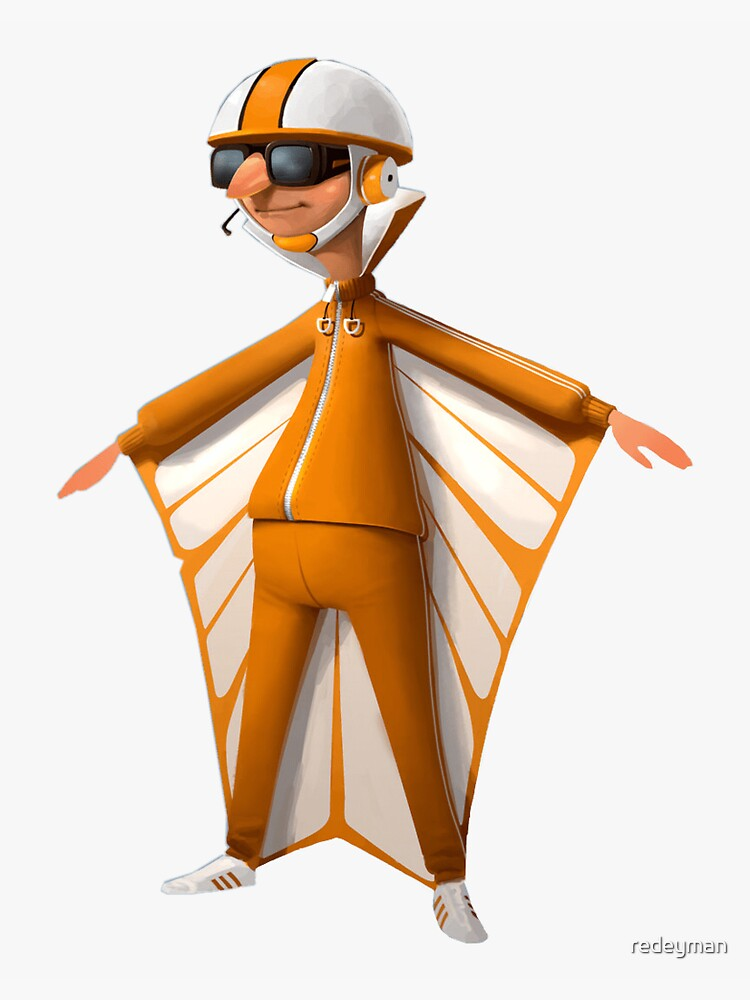
\includegraphics[height=6cm]{vector_d.jpg}
    \end{center}
\end{frame}

\begin{frame}
    \frametitle{What is vector?}
    \begin{block}{Definition}
        Vector: things that are containing both magnitude AND direction\\
        E.g. Force, velocity, acceleration
    \end{block}
    \begin{block}{Type of representation}
        \centering
        \begin{tabular}{|c|c|c|}
            Vector notation & Column vector & Component vector\\
            \hline
            $\vec{AB}$ & $\begin{bmatrix}
                a\\
                b
            \end{bmatrix} $ & $\alpha i + \beta j$
        \end{tabular}
    \end{block}
    Note: We use $O$ to represent origin in Catersian plane, e.g. $\vec{OA}$ = Point of origin (0,0) to point A.\\
    Here, we say A is the position vector (direction relative to the origin)
\end{frame}

\begin{frame}
    \frametitle{Drawing vector}
    \centering
    \begin{tabular}{c c}
        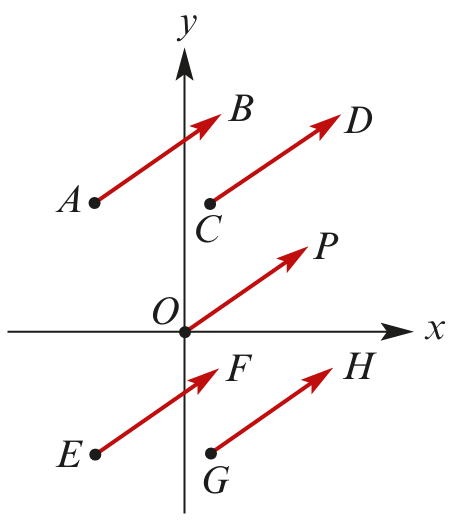
\includegraphics[width = 6cm]{Directed.png} & Note: $\vec{AB} = \vec{CD} = \vec{OP} = \vec{EF} = \vec{GH}$
    \end{tabular}
\end{frame}

\begin{frame}[t]
    \frametitle{Examples}
    \begin{block}{Example 1}
        Draw a directed line segment corresponding to $\begin{bmatrix}
            3 \\ -2
        \end{bmatrix}$
    \end{block}
    \begin{block}{Example 2}
        The vector u is defined by the directed line segment from (2,6) to (3,1).\\
        If $u = \begin{bmatrix}a \\ b\end{bmatrix}$, find $a$ and $b$.
    \end{block}
\end{frame}

\begin{frame}
    \frametitle{Vector addition - Geometric version}
    For column vector, it's like adding matrices. However, how does it look like geometrically?\\
    \begin{center}
        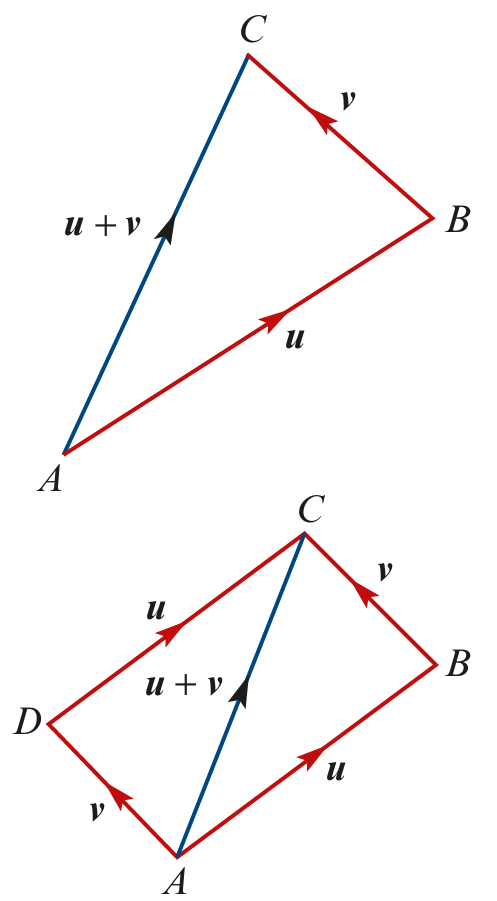
\includegraphics[width = 3.4cm]{Addtion_g.png}
    \end{center}
    Q: What if I want to go from C to A (or $\vec{CA}$)?
\end{frame}

\begin{frame}
    \frametitle{Axioms of vectors}
    Let vectors $u, v, w \in \text{vector space} V$ and $\alpha, \beta \in \mathbb{R}$
    \begin{enumerate}
        \item $u + v = v + u$ (commutative)
        \item $(u + v) + w = u + (v + w)$ (associativity)
        \item There exists a vector $-v$, s.t. $v + (-v) = \vec{0}$ (additive inverse)
        \item $\alpha(\beta v) = (\alpha \beta)v$ (associativity: scalar multiplication)
        \item $1v = v$ (multiplication by unit scalar)
        \item $0v = \vec{0}$
    \end{enumerate}
    \begin{block}{Example 3}
        For the vectors $u = \begin{bmatrix}
            3 \\ -1
        \end{bmatrix}$ and $v = \begin{bmatrix}
            -2 \\ 2
        \end{bmatrix}$, find:
        \begin{enumerate}
            \item $2u + 3v$
            \item $2u - 3v$
        \end{enumerate}
    \end{block}
\end{frame}

\blank

\begin{frame}
    \frametitle{Polygon of vector}
    \begin{center}
        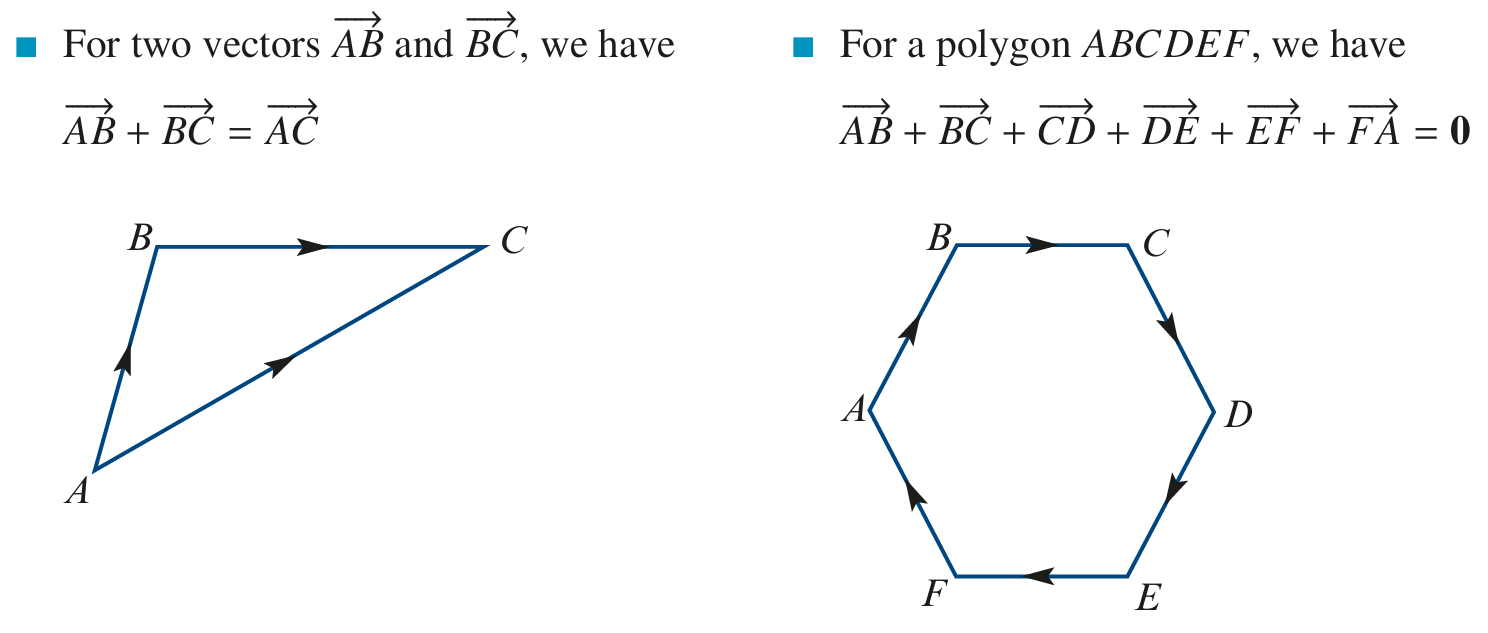
\includegraphics[width = 10cm]{Polygon.png}
    \end{center}
\end{frame}

\begin{frame}[t]
    \frametitle{Parallel vs non-parallel vector}
    \begin{block}{Parallel vector}
        Two non-zero vectors $u$ and $v$ are parallel if there is some $k\in \mathbb{R}$ \textbackslash \{$0$\} such that $u = kv$
    \end{block}
    \begin{block}{Non-parallel vector}
        Let there exists $a \text{and} b$ vectors that are not parallel, then\\
        \begin{center}
            $ma + nb = pa + qb$
        \end{center}        
    \end{block}
    Proof:
\end{frame}
\blank

\begin{frame}
    \frametitle{Parallelograms}
    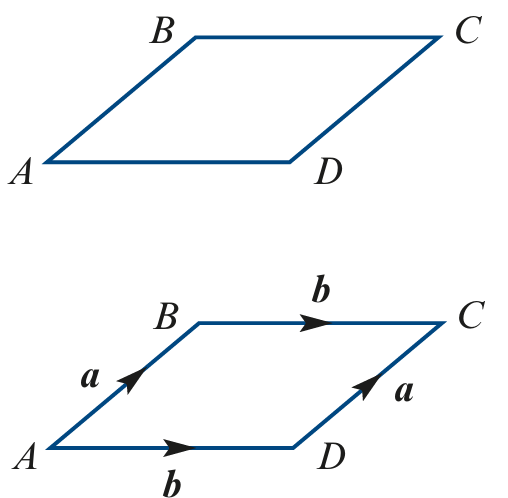
\includegraphics[width = 6cm]{Parallel.png}
\end{frame}

\begin{frame}[t]
    \frametitle{Midpoint example}
    \begin{block}{Example 4}
        Let $A, B \text{ and } C$ be the vertices of a triangles, and let $D$ be the midpoint of $BC$\\
        Let $a = \vec{AB} \text{ and } b = \vec{BC}.$\\
        Find each of the following in terms of $a$ and $b$:\\
        \begin{enumerate}
            \item $\vec{BD}$
            \item $\vec{DC}$
            \item $\vec{AC}$
            \item $\vec{AD}$
            \item $\vec{CA}$
        \end{enumerate}
    \end{block}
\end{frame}
\blank

\begin{frame}[t]
    \frametitle{Harder example}
    \begin{block}{Example 5}
        \begin{multicols}{2}
            In this figure, $\vec{DC} = kp$ where $k\in \mathbb{R} \{0\}$.\\
            \begin{enumerate}
                \item Express $p$ in terms of $k$, $q$ and $r$
                \item Express $\vec{FE}$ in terms of k and p to show that $FE$ is parallel to $DC$
                \item If $\vec{FE} = 4\vec{AB}$, find the value of $k$
            \end{enumerate}
            \columnbreak
            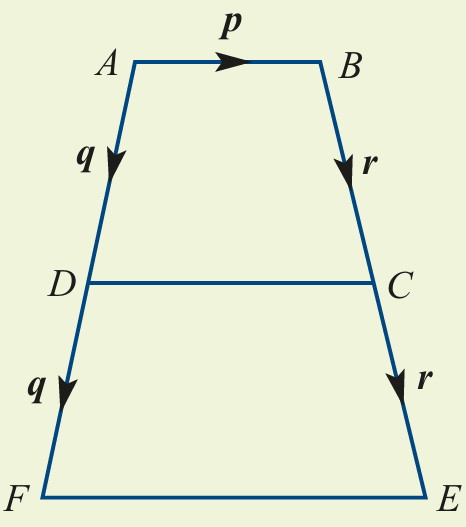
\includegraphics[width = 3cm]{Ex5.png}
        \end{multicols}
    \end{block}
\end{frame}
\blank

\begin{frame}
    \frametitle{Exercise 21A}
\end{frame}

%%%%%%%%%%%%%%%%%%%%%%%%%%%%%%%%%%%%%%%%%%%%%%%%%%%%%%%%%%%%%%%%%%%%%%%%

\section{21B: Component of vectors}
\begin{frame}
    \frametitle{21B}
    \begin{center}
        \title{Component of vectors}
        \maketitle
    \end{center}
\end{frame}

\begin{frame}
    \frametitle{Standard unit vector in $\mathbb{R}^2$}
    \begin{block}{Column vector vs Component vector}
        \[
            \begin{bmatrix}
                1\\0
            \end{bmatrix} = i
            \qquad \begin{bmatrix}
                0\\1
            \end{bmatrix} = j
        \]
    \end{block}
    \begin{block}{Component vector}
        \[
        u = \begin{bmatrix}
            x\\y
        \end{bmatrix} \text{, then: }u = xi + yj.
        \]\\
        Furthermore:\\
        $\text{Magnitude of }u = |u| = \sqrt{x^2 + y^2}$ $\leftarrow$ This is the same as what you learnt in VCE Methods\\
        Note: Some of the other textbooks use $||u||$ to avoid confusion between absolute and magnitude. Hence, if you are using absolute sign in vector 
        it is for magnitude; if it is scalar, it is for absolute.
    \end{block}
\end{frame}

\begin{frame}
    \frametitle{The axioms still work!}
    \begin{enumerate}
        \item $(xi + yj) + (mi + nj) = (x + m)i + (y + n)j$
        \item $k(xi + yj) = kxi + kyi$
        \item Two vectors are equal iff their components are equal:\\
        \begin{center}
            $xi + yi = mi + nj$ iff $x = m \text{ and } y = n$
        \end{center}
    \end{enumerate}
\end{frame}

\begin{frame}[t]
    \frametitle{Example 6}
    \begin{enumerate}
        \item Find $\vec{AB} if \vec{OA} = 3i$ and $\vec{OB} = 2i - j$
        \item Find $|2i - 3j|$
    \end{enumerate}
\end{frame}

\begin{frame}[t]
    \frametitle{Example 7}
    Let $A$ and $B$ be points in the Catersian plane s.t. $\vec{OA} = 2i + j$ and $\vec{OB} = i - 3j$.\\
    Find $\vec{AB}$ and $|\vec{AB}|$.
\end{frame}

\begin{frame}
    \frametitle{Here comes the most confusing part\dots}
    \begin{block}{Unit vector}
        Unit vector is a vector of length one unit\\
        Formula: $\hat{u} = \frac{u}{|u|}$\\
    \end{block}
    What does it actually mean?\\
    Unit vector is to represent any vector that does not have any unit. It always have the length of 1\\
    Why is it important?\\
    This allows us to seperate the magnitude and the direction, hence, we can use it to analyse on the directional properties. \\This is also important 
    we use it in unit cirlce to help us determine angles without calculators!
\end{frame}

\begin{frame}[t]
    \frametitle{Let's try it out}
    \begin{block}{Example 8}
        Let $a = 3i + 4j$\\
        Find $|a|$, the magnitude of $a$, and hence find the unit vector in the direction of $a$.
    \end{block}
\end{frame}

\begin{frame}
    \frametitle{Exercise 21B}
\end{frame}

%%%%%%%%%%%%%%%%%%%%%%%%%%%%%%%%%%%%%%%%%%%%%%%%%%%%%%%%%%%%%%%%%%%%%%%%

\section{21C: Scalar product of vectors}
\begin{frame}
    \frametitle{21C}
    \begin{center}
        \title{Scalar product of vectors}
        \maketitle
    \end{center}
\end{frame}

\begin{frame}
    \frametitle{Scalar product}
    \begin{block}{Definition}
        Scalar (dot) product of two vectors $a = a_i + a_2j$ and $b = b_1i + b2_j$ by\\
    \begin{center}
        $a \cdot b = a_1b_1 + a_2b_2$
    \end{center}
    \end{block}
    $(2i + 3j)\cdot (i-4j) = $\\
    If $a = 0$ or $b = 0$, then $a \cdot b = 0$
\end{frame}

\begin{frame}
    \frametitle{Goemetric description of the scalar product}
    For vectors $a$ and $b$, we have\\
    \begin{center}
        $a \cdot b = |a||b|cos\theta$\\
    \end{center}
    where $\theta$ is the angle between $a$ and $b$.
    \begin{center}
        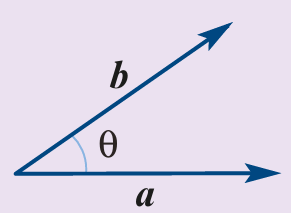
\includegraphics[width = 4cm]{dot_product.png}
    \end{center}
\end{frame}

\begin{frame}[t]
    \frametitle{Understand better}
    Proof:
\end{frame}

\begin{frame}[t]
    \frametitle{Examples}
    \begin{block}{Example 9}
        \begin{enumerate}
            \item If $|a| = 4, |b| = 5$, and the angle between $a$ and $b$ is $30\degree$, find $a\cdot b$.
            \item If $|a| = 4, |b| = 5$, and the angle between $a$ and $b$ is $150\degree$, find $a\cdot b$.
        \end{enumerate}
    \end{block}
\end{frame}

\begin{frame}
    \frametitle{Properties of scalar product}
    \begin{enumerate}
        \item $a\cdot b = b\cdot a$
        \item $k(a\cdot b) = ka\cdot b = a\cdot(kb)$
        \item $a\cdot 0 = 0$
        \item $a\cdot(b+c) = a\cdot b + a\cdot c$
        \item $a\cdot a = |a|^2$
        \item If the vectors $a$ and $b$ are perpendicular, then $a\cdot b = 0$
        \item If $a\cdot b = 0$ for non-zero vectors $a$ and $b$, then the vectors $a$ and $b$ are perpendicular.
    \end{enumerate}
    Note: In more advanced maths, we say $a$ and $b$ are orthogonal if $a\cdot b = 0$. But don't worry, you won't need this.
\end{frame}

\begin{frame}[t]
    \frametitle{Example}
    \begin{block}{Example 10}
        $A, B$ and $C$ are points defined by the position vectors $a,b$ and $c$ respectively, where\\
        \begin{center}
            $a = i + 3j, \qquad b = 2i + j, \qquad c = i - 2j$
        \end{center}       
        Find the magnitude of $\angle ABC$
    \end{block}
\end{frame}

\blank

\begin{frame}
    \frametitle{Exercise 21C}
\end{frame}

%%%%%%%%%%%%%%%%%%%%%%%%%%%%%%%%%%%%%%%%%%%%%%%%%%%%%%%%%%%%%%%%%%%%%%%%

\section{21D: Vector projections}
\begin{frame}
    \frametitle{21D}
    \begin{center}
        \title{Vector projections}
        \maketitle
    \end{center}
\end{frame}

\begin{frame}
    \frametitle{Vector projections}
    Assume there are two vectors $v$ and $u$, where $u \neq 0$, the projection of $v$ onto $u$ is given by:\\
    \begin{center}
        $proj_uv = \frac{u\cdot v}{|u|^2}u = (\hat{u}\cdot v)\hat{u}$\\
        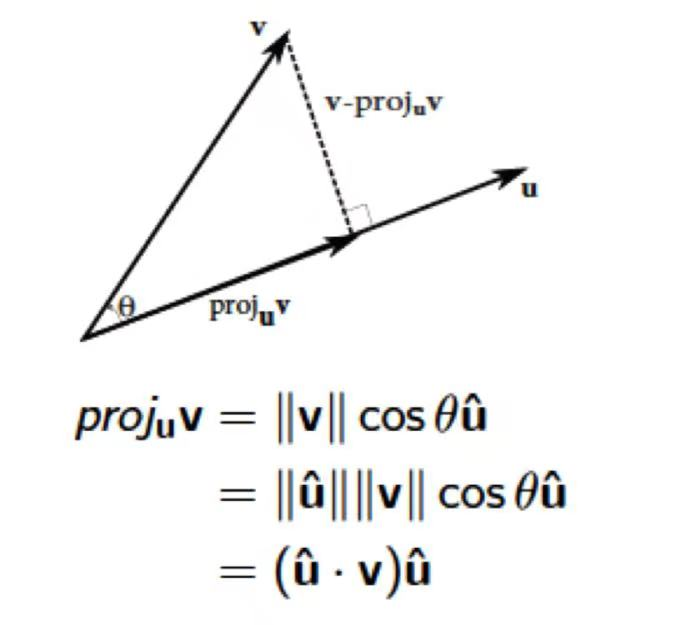
\includegraphics[width = 5cm]{Vector_pro.jpg}
    \end{center}
\end{frame}

\begin{frame}[t]
    \frametitle{Straight to examples}
    \begin{block}{Example 11}
        Let $a = i + 3j$ and $b = i-j$. Find the vector resolute of:
        \begin{enumerate}
            \item $a$ in the direction of $b$
            \item $b$ in the direction of $a$
        \end{enumerate}
    \end{block}
\end{frame}

\begin{frame}[t]
    \frametitle{Straight to examples 2}
    \begin{block}{Example 12}
        Find the scalar resolute of $a = 2i + 2j$ in the direction of $b = -i + 3j$.
    \end{block}
\end{frame}

\begin{frame}[t]
    \frametitle{Straight to examples 3}
    \begin{block}{Example 13}
        Resolve $i + 3j$ into rectangular components, one of which is parallel to $2i- 2j$.
    \end{block}
\end{frame}

\begin{frame}
    \frametitle{Exercise 21D}
\end{frame}

%%%%%%%%%%%%%%%%%%%%%%%%%%%%%%%%%%%%%%%%%%%%%%%%%%%%%%%%%%%%%%%%%%%%%%%%

\section{21E: Geoemetric proofs}
\begin{frame}
    \frametitle{21E}
    \begin{center}
        \title{Geoemetric proofs}
        \maketitle
    \end{center}
\end{frame}

\begin{frame}
    \frametitle{Proofs incoming - but not as scary as before}
    \begin{block}{Definitions to know before proving}
        \begin{enumerate}
            \item Collinear points: Three or more points lie on \textbf{one} single line.
            \item Concurrent lines: Three or more lines lie on \textbf{one} single point.
        \end{enumerate}
    \end{block}
\end{frame}

\begin{frame}
    \frametitle{Also some properties}
    Let there exist vector $\vec{u}$ and $\vec{v}$, and scalar vector $k\in \mathbb{R}^+$ and $\alpha \in \mathbb{R} \textbackslash \{0\}$.
    \begin{block}{Parallel vectors}
        \begin{enumerate}
            \item $k\vec{u}$ has the same direction as $\vec{u}$, and $-k\vec{u}$ has opposite direction. BUT, magnitude are the same here.
            \item For two non-zero vectors $\vec{u}$ and $\vec{v}$ are parallel iff for some $\vec{v}$=$\alpha\vec{u}$
            \item If $\vec{u}$ and $\vec{v}$ are parallel with one point in common, then they lie on the same line
        \end{enumerate}
    \end{block}
    \begin{block}{Scalar products}
        \begin{enumerate}
            \item For two non-zero vectors $\vec{u}$ and $\vec{v}$ are perpendicular iff $\vec{u}\cdot \vec{v} = 0$
            \item $\vec{u}\cdot \vec{u} = |u|^2$
        \end{enumerate}
    \end{block}
\end{frame}

\begin{frame}
    \frametitle{Another one}
    \begin{block}{Linear combinations of non-parallel vectors}
        \begin{enumerate}
            \item For Two non-parallel and non-zero vectors $\vec{u}$ and $\vec{v}$, if  $m\vec{u} + n\vec{v} = p\vec{u} + q\vec{v}$, then\\
            \centering
            $m = p$ \qquad $n = q$
        \end{enumerate}
    \end{block}
\end{frame}

\begin{frame}[t]
    \frametitle{Testing 1 2}
    \begin{block}{Example 14}
        Three points $P, Q$ and $R$ have position vectors $\vec{p}, \vec{q}$ and $k(2\vec{p} + \vec{q})$ respectively, relative to a 
        fixed origin $O$. The points $O, P$ and $Q$ are not collinear. Find the value of $k$ if:\\
        \begin{enumerate}
            \item $\vec{QR}$ is parallel to $\vec{p}$
            \item $\vec{PR}$ is parallel to $\vec{q}$
            \item $P, Q$ and $R$ are collinear.
        \end{enumerate}
    \end{block}
\end{frame}
\blank

\begin{frame}
    \frametitle{Exercise 21E}
\end{frame}

%%%%%%%%%%%%%%%%%%%%%%%%%%%%%%%%%%%%%%%%%%%%%%%%%%%%%%%%%%%%%%%%%%%%%%%%

\section{21F: Application of vectors: displacement and velocity}
\begin{frame}
    \frametitle{21F}
    \begin{center}
        \title{Application of vectors: displacement and velocity}
        \maketitle
    \end{center}
\end{frame}

\begin{frame}
    \frametitle{Important notes: vector vs scalar}
    Recall that:\\
    Vector: things that are containing both magnitude AND direction\\
    Scalar: things that are containing only magnitude\\
    \begin{block}{Vector vs Scalar}
        Vector: displacement, velocity, force.\\
        Scalar: distance, time, speed and mass.
    \end{block}
\end{frame}

\begin{frame}[t]
    \frametitle{Representing displacement with vectors} 
    \begin{block}{Example 15}
        A particle moves from point $A(2,2)$ to point $B(-1,3)$. Express the displacement vector of the particle in component form.
    \end{block}
\end{frame}

\begin{frame}
    \frametitle{What is velocity?} 
    \begin{block}{Definition}
        Velocity: the rate of change of position with respect to time.\\
        What does it mean?\\
        How fast a car can go in respect to time. E.g. If a car can travel 2m in 1s, then we say velocity = $2ms^{-1}$
    \end{block}
    Some velocity representation listed below:\\
    \begin{enumerate}
        \item $80$ $kmh^{-1}$ in the direction north
        \item $10$ $kmh^{-1}$ on a bearing of $080\degree$
        \item $3i + 3j$ $ms^{-1}$
    \end{enumerate}
    \begin{block}{Formula - constant velocity}
        If an object moves with a constant velocity of $v$ $ms^{-1}$ for $t$ seconds, then displacmeent vector, $s$ m:\\
        \begin{center}
            $s = tv$
        \end{center}
    \end{block}
\end{frame}

\begin{frame}[t]
    \frametitle{Apply, apply and apply}
    \begin{block}{Example 16}
        A particle starts at the point $A$ with position vector $\vec{OA} = i + 3j$, where the unit is metres. The particle begins moving 
        with a constant velocity of $2i + 4j ms^{-1}$. Find the position vector of the particle after:\\
        \begin{enumerate}
            \item 5 seconds
            \item $t$ seconds
        \end{enumerate}
    \end{block}
\end{frame}

\begin{frame}[t]
    \frametitle{Apply and apply}
    \begin{block}{Example 17}
        Particle $A$ starts moving from point $O$ with a constant velocity of $v_A = 3i+4j ms^{-1}$. Three seconds after, particle $B$ starts from 
        $O$ and moves in the same directionas $A$ with a constant speed of $7 ms^{-1}$. When and where will $B$ catch up to $A$?
    \end{block}
\end{frame}
\blank

\begin{frame}[t]
    \frametitle{Apply}
    \begin{block}{Example 18}
        A particle starts from $O$ with a constant velocity of $v_1 = 3i + 4j ms^{-1}$. At the same time, a second particle 
        starts moving with constant velocity from the point $B$, where $\vec{OB} = 25j$.\\
        Given that the two particles meet and their paths are at right angles, find:\\
        \begin{enumerate}
            \item the position vector of the point where they meet
            \item the velocity of the second particle
        \end{enumerate}
    \end{block}
\end{frame}
\blank

\begin{frame}
    \frametitle{Exercise 21F}
\end{frame}

%%%%%%%%%%%%%%%%%%%%%%%%%%%%%%%%%%%%%%%%%%%%%%%%%%%%%%%%%%%%%%%%%%%%%%%%

\section{21G: Application of vectors: relative velocity}
\begin{frame}
    \frametitle{21G}
    \begin{center}
        \title{Application of vectors: relative velocity}
        \maketitle
    \end{center}
\end{frame}

\begin{frame}[t]
    \frametitle{Resultant velocity}
    Resultant is the sume all vectors. $\therefore$ Resultant velocity is all velocity vectors summing up!\\
    \begin{block}{Example 19}
        A river is flowing north at $5kmh^1$. Mila can swim at $2kmh^{-1}$ in still water. She dives in from the west bank of the river 
        and swim towards the oppsite bank.
        \begin{enumerate}
            \item In which direction does she travel?
            \item What is her actual speed?
        \end{enumerate}
    \end{block}
\end{frame}
\blank

\begin{frame}
    \frametitle{Things are getting saucy here}
    Relative velocity: velocity that is relative from one things to another.\\
    From example above: We are able to conclude\\
    $v_{s|b} = v_{s|w} + v_{w|b}$\\
    General formula: $v_{a|b} = v_a - v_b$\\
    If we are measuring according to Earth or sometimes origin, this is called \textbf{true velocities} or \textbf{actual velocities}
\end{frame}

\begin{frame}[t]
    \frametitle{Make some relative motions}
    \begin{block}{Example 20}
        A train is moving with a constant velocity of $80 kmh^{-1}$ north. A passenger walks straight
 across a carriage from the west side to the east side at $3 kmh^{-1}$. What is the true velocity of
 the passenger?
    \end{block}
\end{frame}
\blank

\begin{frame}[t]
    \frametitle{Another one}
    \begin{block}{Example 21}
        Car A is moving with a velocity of $50 kmh^{-1}$ due north, while car B is moving with a
        velocity of $120 kmh^{-1}$ due west. What is the velocity of car A relative to car B?
    \end{block}
\end{frame}
\blank

\begin{frame}[t]
    \frametitle{Jet incoming}
    Note: \alert{Airspeed}: speed relative to air
    \begin{block}{Example 22}
        A light aircraft has an airspeed of $250 kmh^{-1}$. The pilot sets a course due north. If the
        wind is blowing from the north-west at $80 kmh^{-1}$, what is the true speed and direction of
        the aircraft?
    \end{block}
\end{frame}
\blank

\begin{frame}[t]
    \frametitle{Another one}
    \begin{block}{Example 23}
        An aeroplane is scheduled to travel from a point P to a point Q, which is $1000 km$
        due west of P. The aeroplane's airspeed is $500 kmh^{-1}$ and the wind is blowing from the
        south-west at $100 kmh^{-1}$.
        \begin{enumerate}
            \item In which direction should the pilot set the course?
            \item How long will the flight take?
        \end{enumerate}
    \end{block}
\end{frame}
\blank

\begin{frame}
    \frametitle{Exercise 21G}
\end{frame}

%%%%%%%%%%%%%%%%%%%%%%%%%%%%%%%%%%%%%%%%%%%%%%%%%%%%%%%%%%%%%%%%%%%%%%%%

\section{21H: Application of vectors: forces and equilibrium}
\begin{frame}
    \frametitle{21H}
    \begin{center}
        \title{Application of vectors: forces and equilibrium}
        \maketitle
    \end{center}
\end{frame}

\begin{frame}
    \frametitle{Physicists' favourite}
    We now introduce forces, where it is always using $F=ma$.\\
    However, when solving forces, we always need to consider where the equilibrium is at.\\
    \begin{block}{Normal Force}
        \centering
        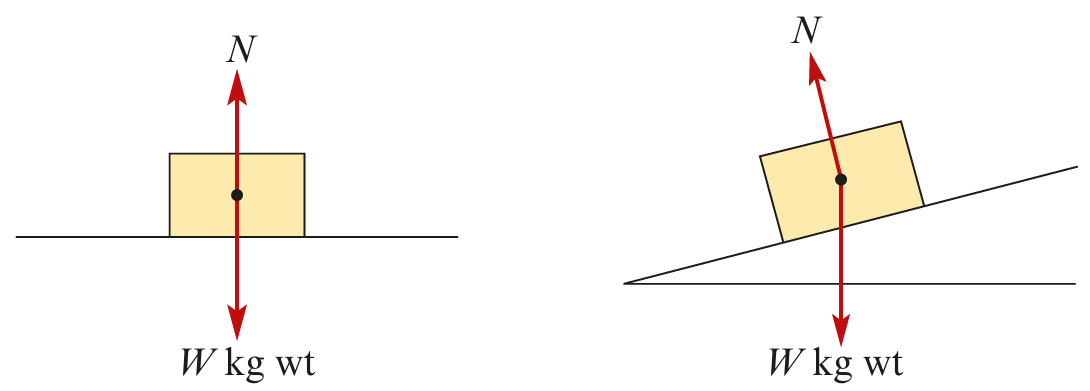
\includegraphics[width = 6cm]{Normal}
    \end{block}
\end{frame}

\begin{frame}
    \frametitle{Tension force}
    \centering
    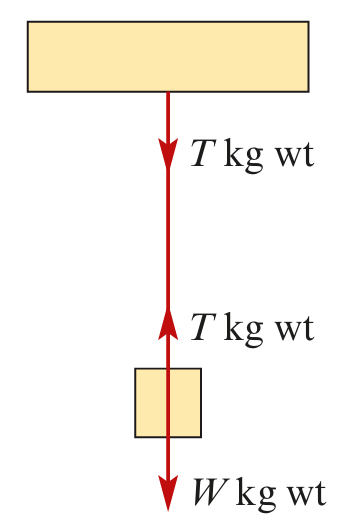
\includegraphics[width = 4cm]{Tension.png}
\end{frame}

\begin{frame}
    \frametitle{Tension force}
    \centering
    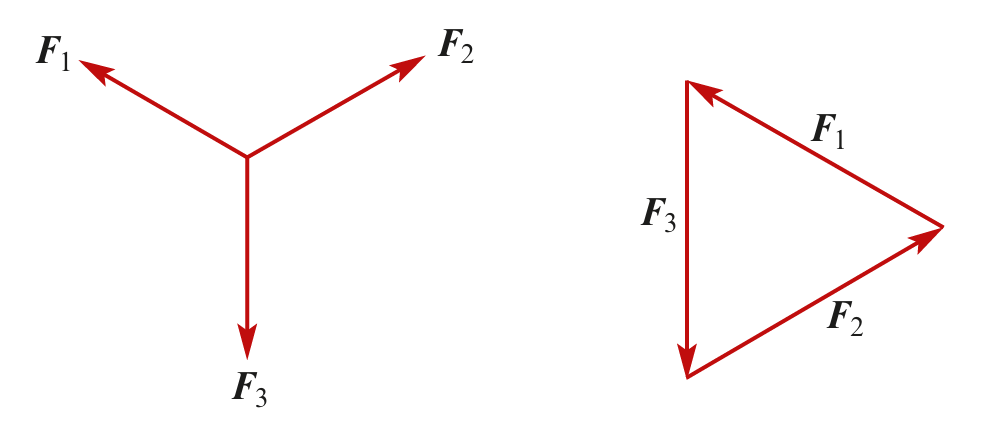
\includegraphics[width = 8cm]{Triangle.png}
\end{frame}

\begin{frame}[t]
    \frametitle{Examples}
    \begin{block}{Example 24}
        A particle of mass 8kg is suspended by two strings attached to two points in the same horizontal plane. 
        If the two strings make angles of $30\degree$ and $40\degree$ to the horizontal, find the tension in each string.
    \end{block}
\end{frame}
\blank

\begin{frame}[t]
    \frametitle{Example 25}
    A particle of mass 15 kg is suspended vertically from a point P by a string. The particle is pulled horizontal by 
    a force of F kg wt so that the string makes an angle of $30degree$ with the vertical.\\
    Find the value of F and the tension of string.
\end{frame}
\blank

\begin{frame}[t]
    \frametitle{Example 26}
    A body mass 20kg is placed on a smooth plane inclined at $30\degree$ to the horizontal. A string is attached to a point 
    further up the plane which prevents the body from moving. Find the tension in the string and the magnitude of the force exerted on the body by the plane.
\end{frame}
\blank

\begin{frame}
    \frametitle{Resolution of forces}
    \begin{center}
        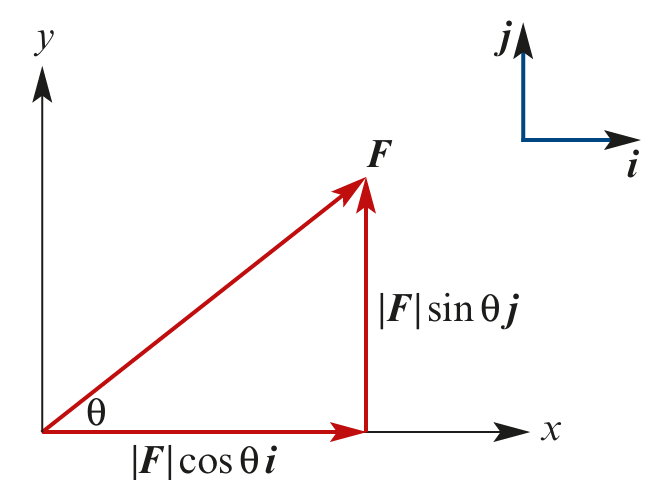
\includegraphics[width = 4cm]{Resolution.png}
    \end{center}
    $F = |F|cos\theta i + |F|sin\theta j$\\
    \alert{If the particle is in equilibrium, then sum of all $i$ or $j$ components are zero}
\end{frame}

\begin{frame}[t]
    \frametitle{Example 27}
    A particle of mass 8kg is suspended by two strings attached to two points in the same horizontal plane. If the two strings make angle of $30\degree$ and 
    $60\degree$ to the horizontal, find the tension in each string.
\end{frame}
\blank

\begin{frame}[t]
    \frametitle{Example 28}
    A body of mass 10kg is held at rest on a smooth plane inclined at $20\degree$ by a string with tension 5kg wt.\\
    Find an angle between string and the inclined plane.
\end{frame}
\blank

\begin{frame}
    \frametitle{Exercise 21H}
\end{frame}

%%%%%%%%%%%%%%%%%%%%%%%%%%%%%%%%%%%%%%%%%%%%%%%%%%%%%%%%%%%%%%%%%%%%%%%%

\section{21I: Vectors in three dimensions}
\begin{frame}
    \frametitle{21I}
    \begin{center}
        \title{Vectors in three dimensions}
        \maketitle
    \end{center}
\end{frame}

\begin{frame}
    \frametitle{Same format but with $k$}
    \begin{block}{Type of representation}
        \centering
        \begin{tabular}{|c|c|c|}
            Vector notation & Column vector & Component vector\\
            \hline
            $\vec{AB}$ & $\begin{bmatrix}
                a\\
                b\\
                c
            \end{bmatrix} $ & $\alpha i + \beta j + \gamma k$
        \end{tabular}
    \end{block}
\end{frame}

\begin{frame}[t]
    \frametitle{More on vector}
    \begin{center}
        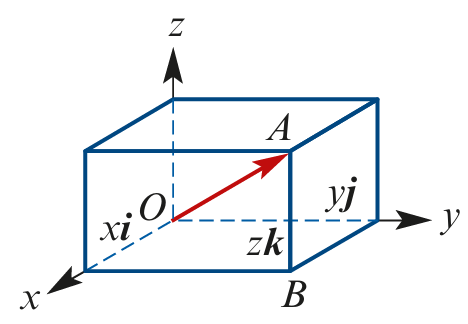
\includegraphics[width = 4cm]{3d.png}
    \end{center}
    $\vec{OA}^2 = \vec{OB}^2 + \vec{BA}^2$ (continue to derive)
\end{frame}

\begin{frame}[t]
    \frametitle{Example 29}
    Let $a = i + j - k$ and $b = i + 7k$. Find:\\
    \begin{enumerate}
        \item $a + b$
        \item $b-3a$
        \item $|a|$
    \end{enumerate}
\end{frame}

\begin{frame}[t]
    \frametitle{Example 30}
    $OABCDEFG$ is a cuboid s.t.$\vec{OA} = 3j$, $\vec{OC} = k$ and $\vec{OD} = i$.\\
    \begin{enumerate}
        \item Express each of the following in terms of $i$, $j$, and $k$:
        \begin{enumerate}
            \item $\vec{OE}$
            \item $\vec{OF}$
            \item $\vec{GF}$
            \item $\vec{GB}$
        \end{enumerate}
        \item Let $M$ and $N$ be the midpoints of $OD$ and $GF$ respectively. Find $MN$.
    \end{enumerate}
\end{frame}
\blank

\begin{frame}[t]
    \frametitle{Example 31}
    If $a = 3i + 2j + 2k$, find $\hat{a}$.
\end{frame}

\begin{frame}
    \frametitle{Exercise 21I}
\end{frame}

\end{document}